% !TEX root = ../algorithms.tex

\section{Префиксные суммы (префиксное накопление, операция \texttt{scan}). Сумматор Ладнера--Фишера.}

\textbf{Задача (prefix sums).}
Построить вычислительную схему, которая принимает на вход
$n$ чисел $x_0,\dots,x_{n-1}$ и (используя только бинарную операцию ``$+$'')
выдаёт числа $y_0,\dots,y_{n-1}$, где
\[
y_i=\sum_{j=0}^{i} x_j,\qquad i=0,\dots,n-1.
\]

\subsection*{Схема Ладнера--Фишера}

Пусть $n$ чётное.

Сначала попарно складываем входы:
\[
s_i=x_{2i}+x_{2i+1},\qquad i=0,\dots,\frac{n}{2}-1.
\]
Рекурсивно считаем префиксные суммы для $s$:
\[
p_i=\sum_{j=0}^{i}s_j.
\]
Тогда выходы восстанавливаются так:
\[
y_{2i+1}=p_i,\qquad
y_{2i}=
\begin{cases}
	x_0, & i=0,\\
	p_{i-1}+x_{2i}, & i\ge 1.
\end{cases}
\]

\begin{figure}[h]
	\centering
	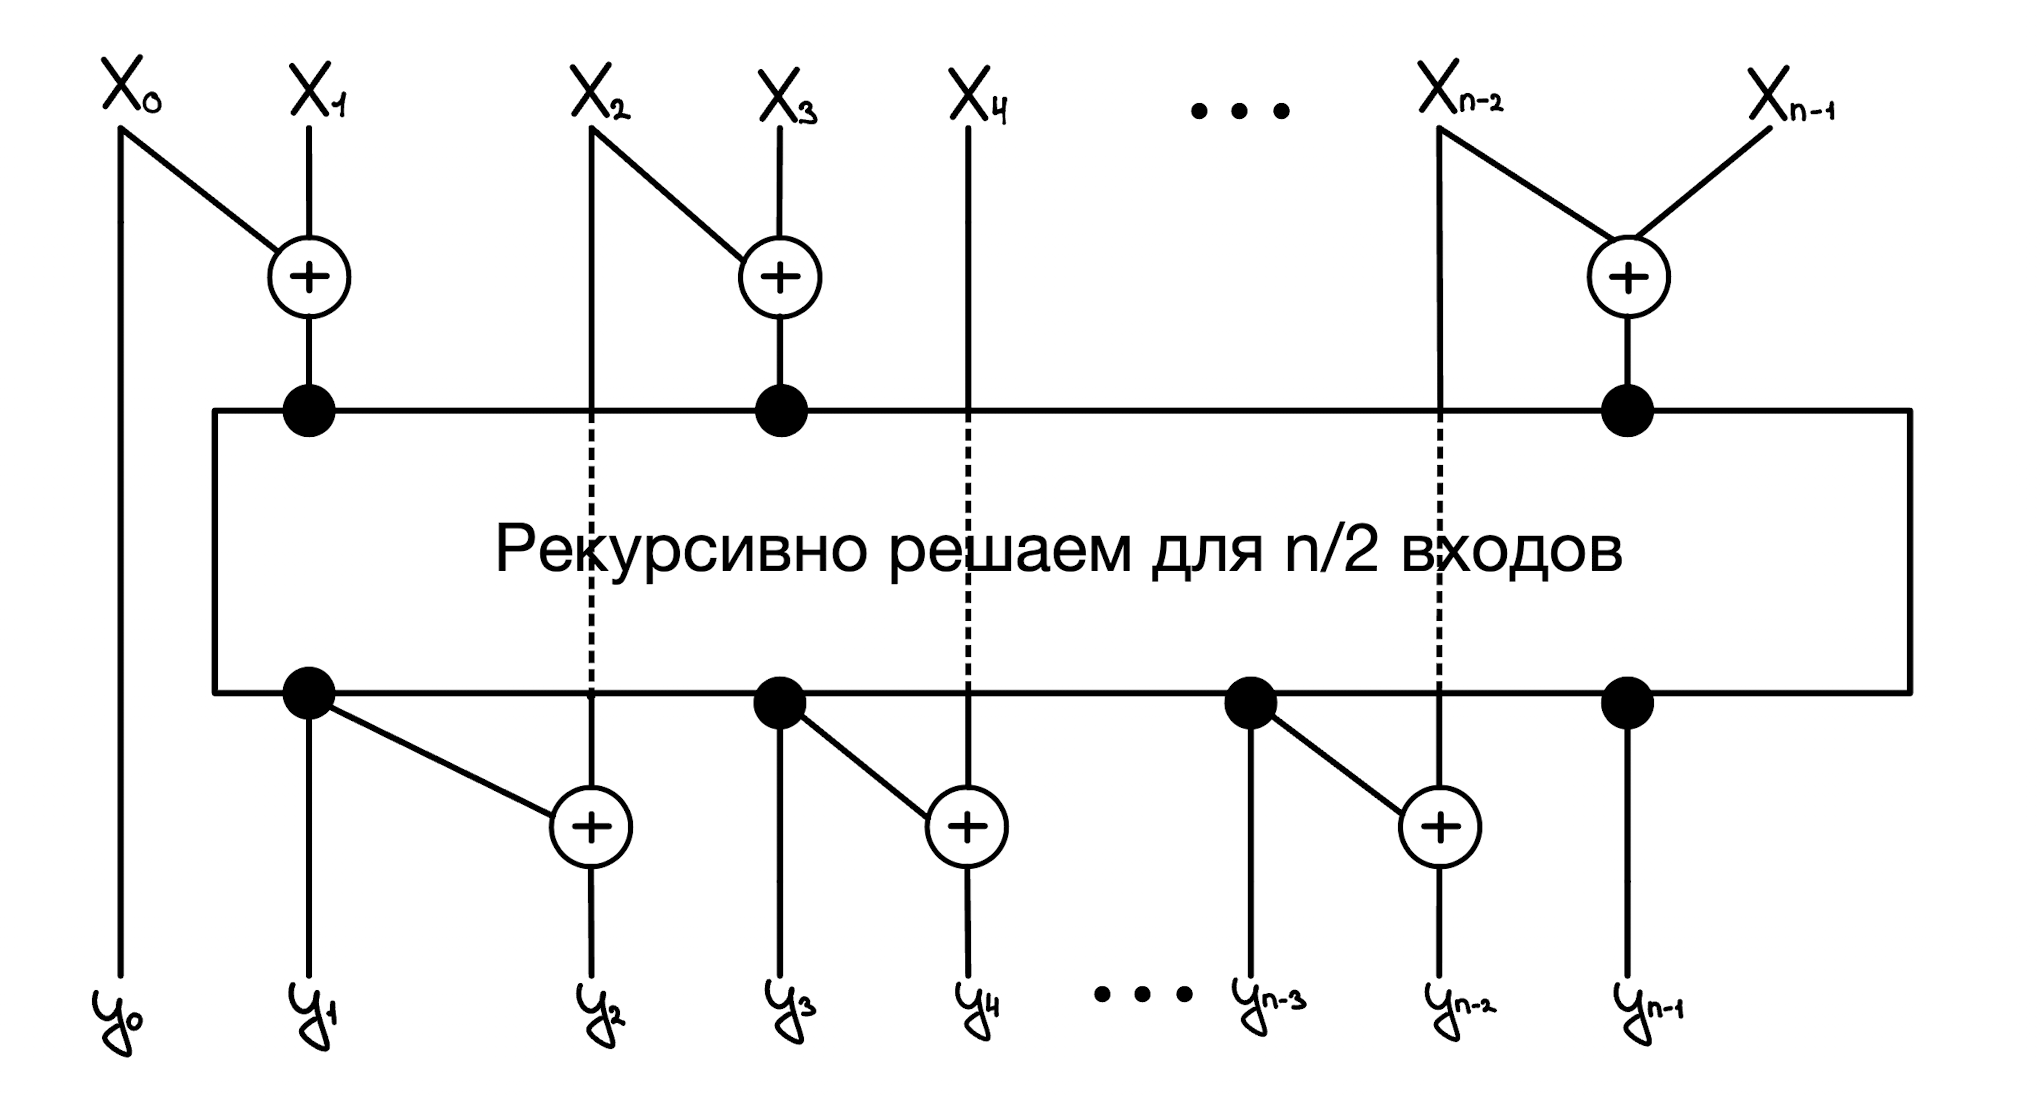
\includegraphics[width=0.8\textwidth]{img/ladner-fischer.png}
	\caption{Схема Ладнера--Фишера для префиксных сумм}
	\label{fig:ladner-fischer}
\end{figure}

\paragraph{Оценки (глубина и размер).}
\[
T(n)=2+T\!\left(\frac{n}{2}\right)=2\log_2 n,\qquad
S(n)=n+S\!\left(\frac{n}{2}\right)=2n-2.
\]
Идея хорошо ложится на GPU (много независимых операций на каждом уровне).

\paragraph{Замечание.}
Операция \texttt{scan} — базовый блок для разработки параллельных алгоритмов.
Вместо ``$+$'' можно использовать любую \textbf{ассоциативную} операцию $\odot$:
\[
y_i=x_0\odot x_1\odot\cdots\odot x_i.
\]
Примеры ассоциативных структур:
\[
(\{0,1\},\ \vee,\ \wedge),\qquad
(\{0,1\},\ \wedge,\ \vee),\qquad
(\mathbb{R},\ \min,\ +).
\]

\subsection*{Псевдокод \texttt{scan}}

Пусть $n=2^m$.

\begin{algorithm}[H]
	\caption{\texttt{scan} (in-place), inclusive, по доске}
	\begin{algorithmic}[1]
		\Require массив $x[0..n-1]$, где $n=2^m$
		\Comment{Upsweep: накапливаем суммы на концах блоков}
		\For{$d=0$ \textbf{to} $\log_2 n - 1$}
		\For{$k=0$ \textbf{to} $n-1$ \textbf{step} $2^{d+1}$}
		\State $x[k+2^{d+1}-1] \gets x[k+2^{d+1}-1] + x[k+2^{d}-1]$
		\EndFor
		\EndFor
		\Comment{Downsweep: добавляем префикс предыдущего блока к левому подблоку}
		\For{$d=\log_2 n - 1$ \textbf{downto} $0$}
		\For{$k=0$ \textbf{to} $n-1$ \textbf{step} $2^{d+1}$}
		\If{$k>0$}
		\State $x[k+2^{d}-1] \gets x[k+2^{d}-1] + x[k-1]$
		\EndIf
		\EndFor
		\EndFor
	\end{algorithmic}
\end{algorithm}

\begin{Example}{Сведения к \texttt{scan}: рекурсия вида $c_{k+1}=a_k+b_k c_k$}{}
Даны числа $a_0,\dots,a_{n-1}$ и $b_0,\dots,b_{n-1}$.
Нужно найти $c_0,\dots,c_n$ такие, что
\[
c_0=0,\qquad c_{k+1}=a_k+b_k\,c_k.
\]

Определим строковый вектор
\[
C_k=(1,\ c_k).
\]
Тогда
\[
C_{k+1}=C_k\,X_k,\qquad
X_k=
\begin{pmatrix}
	1 & a_k\\
	0 & b_k
\end{pmatrix}.
\]
Отсюда
\[
C_1=C_0X_0,\quad
C_2=C_0X_0X_1,\quad
C_3=C_0X_0X_1X_2,\ \dots
\]
То есть достаточно посчитать префиксные произведения матриц $X_0,X_1,\dots,X_{n-1}$
(умножение матриц ассоциативно), и это делается через \texttt{scan} за
$O(\log n)$ времени в параллельной модели.
\end{Example}

\subsection*{Сумматор Ладнера--Фишера и переносы}

\begin{Definition}{}{}
\textbf{Сумматор} — это вычислительная схема над булевыми операциями
$(\vee,\wedge,\oplus,\neg,\dots)$, которая принимает на вход биты
\[
x_0,\dots,x_{n-1},\qquad y_0,\dots,y_{n-1}
\]
и выдаёт биты
\[
z_0,\dots,z_n
\]
такие, что $z=x+y$, где
\[
x=\sum_{k=0}^{n-1}x_k2^k,\qquad
y=\sum_{k=0}^{n-1}y_k2^k,\qquad
z=\sum_{k=0}^{n}z_k2^k.
\]
\end{Definition}

\subsection*{Биты переноса и сведение к \texttt{scan}}

Пусть $c_k$ — перенос \emph{в} разряд $k$ (по определению $c_0=0$).
Тогда для $k=0,\dots,n-1$ выполняется формула переноса:
\[
c_{k+1}=(x_k\wedge y_k)\ \vee\ (x_k\wedge c_k)\ \vee\ (y_k\wedge c_k).
\]
Её удобно переписать в виде
\[
c_{k+1}=a_k\ \vee\ (b_k\wedge c_k),
\qquad
a_k:=x_k\wedge y_k,\quad b_k:=x_k\vee y_k.
\]
Если все переносы $c_0,\dots,c_n$ известны, то ответ восстанавливается по формулам
\[
z_k=x_k\oplus y_k\oplus c_k\quad (k=0,\dots,n-1),
\qquad
z_n=c_n.
\]

\medskip
\textbf{Ключевая идея:} рекуррента
\[
c_{k+1}=a_k\ \vee\ (b_k\wedge c_k)
\]
имеет вид ``аффинного'' преобразования, которое можно упаковать в матрицу.
Положим
\[
C_k=(1,\ c_k),\qquad
X_k=
\begin{pmatrix}
	1 & a_k\\
	0 & b_k
\end{pmatrix}.
\]
Тогда
\[
C_{k+1}=C_kX_k,
\]
где операции в матрице понимаются над булевым полукольцом $(\{0,1\},\ \vee,\ \wedge)$.
Следовательно, нужно посчитать префиксные произведения
\[
C_k=C_0X_0X_1\cdots X_{k-1},
\]
что делается через \texttt{scan} за $O(\log n)$ времени (в параллельной модели).

\subsection*{Замечание про \texttt{scan}}
Для \texttt{scan} не нужно именно кольцо $(\mathbb{R},+,\cdot)$:
достаточно ассоциативной операции (моноида), а для матричной записи удобно полукольцо.

\subsection*{Модель PRAM}

\begin{Definition}{}{}
\textbf{PRAM} (Parallel Random Access Machine) — идеализированная модель параллельных вычислений:
\begin{itemize}
	\item есть \textbf{общая глобальная память};
	\item есть (теоретически) \textbf{неограниченное число процессоров},
	каждый процессор — RAM с собственным номером $p=1,2,\dots$;
	\item процессоры работают \textbf{синхронно}: за единицу времени выполняют одну инструкцию.
\end{itemize}
\end{Definition}

\subsection*{Разрешение конфликтов доступа к памяти}

Для чтения/записи различают режимы \textbf{concurrent/exclusive}:
\begin{itemize}
	\item \textbf{concurrent read} — несколько процессоров могут одновременно читать одну ячейку;
	\item \textbf{concurrent write} — несколько процессоров могут одновременно писать в одну ячейку;
	в модели CRCW нужно отдельно задавать правило разрешения конфликта
	(например, \emph{arbitrary}: остаётся одно из записанных значений);
	\item \textbf{exclusive} — если несколько процессоров обращаются к одной ячейке ``одновременно'',
	это запрещено (поведение не определено/``мусор'').
\end{itemize}

\textbf{Стандартные варианты PRAM:}
\[
\text{CRCW PRAM},\quad
\text{CREW PRAM},\quad
\text{ERCW PRAM},\quad
\text{EREW PRAM}.
\]

\subsection*{Класс NC}

\textbf{NC} — класс задач, которые решаются на PRAM за время $(\log n)^{O(1)}$
при использовании \emph{полиномиального} числа процессоров $n^{O(1)}$.

\subsection*{Как в PRAM посчитать \texttt{scan} на $p$ процессорах}

Пусть дан массив $A[0..n-1]$ и $p$ процессоров. Разобьём массив на блоки длины
$m=n/p$ (для простоты считаем $p\mid n$).

\begin{enumerate}
	\item Каждый процессор $i$ считает \textbf{локальный scan} на своём блоке
	$A[im..(i+1)m-1]$ последовательно за время $O(m)=O(n/p)$.
	Обозначим сумму блока как $T_i$ (последний элемент локального scan).
	\item Считаем \textbf{scan по массиву блок-сумм} $T_0,T_1,\dots,T_{p-1}$ за время $O(\log p)$.
	Пусть
	\[
	P_i=\sum_{j=0}^{i-1} T_j
	\]
	— сумма всех предыдущих блоков (смещение для блока $i$).
	\item Каждый процессор прибавляет смещение $P_i$ ко всем элементам своего блока
	(снова $O(n/p)$ времени).
\end{enumerate}

Итого время:
\[
O\!\left(\frac{n}{p}+\log p\right).
\]
В частности, при $p=\Theta\!\left(\frac{n}{\log n}\right)$ получаем $O(\log n)$ времени.

\begin{Example}{Сортировка подсчётом (Counting sort) в PRAM}{}
Дан массив $a[0..n-1]$, причём $a[k]\in\{0,\dots,U\}$, где $U=O(1)$.
Есть $p$ процессоров, каждый обрабатывает блок длины $n/p$.

\begin{itemize}
	\item Процессор $i$ строит таблицу частот $c_i[0..U]$, где
	\[
	c_i(x)=\#\{\,k\in[im,(i+1)m-1]\mid a[k]=x\,\},
	\qquad m=\frac{n}{p}.
	\]
	Это занимает $O(n/p)$ времени.
	\item Далее частоты суммируются по процессорам (для каждого $x$ делается редукция),
	затем берутся префиксные суммы по $x$, и заполняется выходной массив.
	Так как $U=O(1)$, вся работа по значениям $x$ остаётся константной.
\end{itemize}
\end{Example}